% !TEX program = xelatex
\documentclass[10pt,twocolumn,a4paper]{article}

% ---------------------------------------------------------------------------
%  Formato: el enunciado no nombra ninguna plantilla de congreso. Pide
%  «4-6 pages» y que «should, in principle, look similar to a typical research
%  paper in the field of NLP». Esto imita el estilo *ACL: A4 a dos columnas,
%  Times (Liberation Serif es métricamente compatible), resumen en bloque
%  estrecho, secciones numeradas en negrita.
% ---------------------------------------------------------------------------

\usepackage{fontspec}
\setmainfont{LiberationSerif}[
  Path = /usr/share/fonts/truetype/liberation/,
  Extension = .ttf, UprightFont = *-Regular, BoldFont = *-Bold,
  ItalicFont = *-Italic, BoldItalicFont = *-BoldItalic]
\setsansfont{LiberationSans}[
  Path = /usr/share/fonts/truetype/liberation/,
  Extension = .ttf, UprightFont = *-Regular, BoldFont = *-Bold,
  ItalicFont = *-Italic, BoldItalicFont = *-BoldItalic]
\setmonofont{LiberationMono}[
  Path = /usr/share/fonts/truetype/liberation/,
  Extension = .ttf, UprightFont = *-Regular, BoldFont = *-Bold,
  ItalicFont = *-Italic, BoldItalicFont = *-BoldItalic, Scale = 0.85]

\usepackage[a4paper,left=2cm,right=2cm,top=2.5cm,bottom=2cm,
            columnsep=0.2in]{geometry}
\usepackage{amsmath,amssymb}
\usepackage{booktabs}
\usepackage{microtype}
\usepackage{xcolor}
\usepackage{titlesec}
\usepackage{caption}
\usepackage{pgfplots}
\pgfplotsset{compat=1.18}
\usepackage[hidelinks]{hyperref}
% la URL de la nota al pie no tiene guiones donde partir: deja que hyperref
% rompa por cualquier carácter, si no desborda la columna por 2 pt
\def\UrlBreaks{\do\/\do-\do.\do_\do a\do b\do c\do d\do e\do f\do g\do h\do i%
\do j\do k\do l\do m\do n\do o\do p\do q\do r\do s\do t\do u\do v\do w\do x%
\do y\do z\do A\do B\do C\do D\do E\do F\do G\do H\do I\do J\do K\do L\do M%
\do N\do O\do P\do Q\do R\do S\do T\do U\do V\do W\do X\do Y\do Z}
\Urlmuskip=0mu plus 1mu

\captionsetup{font=small,labelfont=bf,skip=4pt}
\titleformat{\section}{\large\bfseries}{\thesection}{0.6em}{}
\titleformat{\subsection}{\normalsize\bfseries}{\thesubsection}{0.6em}{}
\titlespacing*{\section}{0pt}{11pt}{4pt}
\titlespacing*{\subsection}{0pt}{8pt}{3pt}
\titlespacing*{\paragraph}{0pt}{6pt plus 1pt minus 1pt}{0.6em}
\setlength{\textfloatsep}{12pt plus 2pt minus 2pt}
\setlength{\floatsep}{10pt plus 2pt minus 2pt}
\setlength{\parskip}{0pt}
\raggedbottom
\setlength{\abovedisplayskip}{6pt}
\setlength{\belowdisplayskip}{6pt}

\newcommand{\tec}[1]{{\small\texttt{#1}}}

% resumen al estilo ACL: bloque estrecho en la primera columna
\newenvironment{aclabstract}
  {\begin{center}\large\bfseries Abstract\end{center}\vspace{-2pt}%
   \begingroup\leftskip=0.45cm\rightskip=0.45cm\small}
  {\par\endgroup\vspace{6pt}}

\title{\vspace{-1.4cm}\LARGE\bfseries Does adaptation compose?\\[3pt]
\large Independently trained language and genre modules\\
on a low-resource intersection domain}
\author{\normalsize Marcos Lahoz}
\date{}

\begin{document}
\maketitle

\begin{aclabstract}
\noindent
Domains that matter for the humanities sit at intersections of language, period
and genre where almost no text exists, while the margins that contain them are
data-rich. We ask whether adaptation to such a cell can be assembled from
modules trained independently on those margins, and test it for a language
factor and a genre factor on $\langle$Swedish, literary$\rangle$. The design
forces a confound we make central: to keep the target unseen, neither module can
be trained on its factor alone. The consequence is stark --- neither module helps the
target by itself, and their plain sum is worse than doing nothing --- and yet
averaging them helps, with no target data at all. What governs the composition
turns out to be the \emph{magnitude} of the two updates rather than their
\emph{direction}: three probes across two different spaces recover almost
nothing, while one fitted scalar per module does the work.
\end{aclabstract}

\section{Introduction}

A concrete text domain is rarely defined by a single property. A 17th-century
Dutch pamphlet and a contemporary Icelandic court ruling differ in language, in
period and in genre simultaneously. Suppose a set of natural languages $L$, a
set of periods $P$ and a set of genres $G$: a domain is a cell $\langle
l,p,g\rangle$ of the grid $|L|\times|P|\times|G|$, and the cells that matter for
the humanities are usually close to empty, while the marginals that contain them
are not. Those marginals are
what one can actually train on. This is the situation the ELMA project
addresses: if the adaptation of a language model to a cell could be decomposed
into contributions from each dimension, one could learn each contribution where
data is plentiful and assemble a cell that was never observed.

Whether the factors of a humanities domain compose at all is an open question,
and they may not: the variation of an intersection domain may have an
irreducible structure of its own, not recoverable from its margins. We therefore organise the study around explaining
an outcome rather than around demonstrating a method: we adapt a multilingual backbone independently to a
language factor and to a genre factor, compose the two resulting modules on the
intersection cell, and measure. The cell reported here is $\langle$Swedish,
literary$\rangle$.\footnote{Code, the notebook with its saved outputs, the full
training configuration and the corpus measurements:
\url{https://github.com/mlahozy21/Modular-and-Compositional-Adaptation-of-a-Multilingual-LM}}

\paragraph{Neither module can be trained on its factor alone.}
This is forced by the design. To keep the target cell unseen, the genre module can
only be trained on the target genre in \emph{other} languages, and the language
module on the target language in the \emph{other} genre.
Here the ``language'' module is
trained on legal Swedish and therefore encodes \emph{legal} Swedish; the
``genre'' module is trained on literary text in fifteen languages none of which
is Swedish, and therefore encodes literary \emph{non-Swedish}.

Composing is therefore not adding two clean directions; it is
adding two mixtures and hoping the unwanted halves cancel. It also makes a
negative result ambiguous by default --- the factors may fail to compose, or the
confounds may compose badly --- and separating those two readings is a design
problem. Section~\ref{sec:interp} measures the confound directly.

\section{Background and setting}

\label{sec:why}

We use two datasets, both parallel corpora distributed through the HuggingFace
Hub and organised as language pairs.

\tec{Helsinki-NLP/opus\_dgt} is the legal half: the Translation Memory of the
European Commission's Directorate-General for Translation, i.e.\ EU legislation
drafted once and translated into the official languages, and therefore
formulaic, templatic, and built from the same source documents in every
language. The copy on the Hub covers 10 languages, not the 25 the dataset card
declares. \tec{Helsinki-NLP/opus\_books} is the literary half: out-of-copyright
novels and their translations, four times smaller, far more varied in style and
far more unevenly spread across languages. As published on the Hub, \tec{opus\_books} covers 16 languages and 49.0M words,
of which 0.20M are Swedish, and \tec{opus\_dgt} 10 languages and 195.0M words, of
which 11.14M are Swedish; words are whitespace-separated and counted over every
pair containing the language, so repetitions across pairs are counted.
\emph{Genre} therefore takes exactly two values here, and the period dimension of
the general ELMA framing is not exercised.

\paragraph{The admissible grid is forced, not chosen.}
A cell $\langle l,g\rangle$ is usable only if $l$ appears in \emph{both}
datasets: the genre module needs the other languages within the target genre,
and the language module needs the target language within the other genre. The
intersection of the two language inventories is four languages --- Swedish,
Finnish, Dutch, Spanish --- giving $4\times 2 = 8$ admissible cells. Every
design decision below is a choice among eight, not among four hundred.

\paragraph{Why Swedish.} Of the four, Swedish fits the project best, for two
reasons.

First, the target cell is scarce: the entire Swedish literary portion is
199{,}605 words, 0.41\% of the literary corpus, against 3{,}657{,}410 for Dutch
and 7{,}008{,}693 for Spanish. That single slice \emph{is} the target cell,
training, validation and test together. One qualification: it is the smallest of the four by raw count, but the
ranking against Finnish (254{,}346) reverses once repetition is removed. Each
slice is one work in several translation pairs --- three for Swedish, six for
Finnish --- and on exact-deduplicated text the Swedish slice is 75{,}763 words
against 67{,}703 Finnish. Exact deduplication is a lower bound on the
repetition, since differing segmentations leave near-copies intact. The scarcity argument
holds against Dutch and Spanish by more than an order of magnitude; against
Finnish it does not, and the case for this cell rests on the reason that
follows.

Second, the modules can be trained on comparable, if not equal, amounts: 11.14M
words of legal Swedish against 48.60M of literary non-Swedish, a ratio of $4.4$
where the Finnish cell gives 2.85M against 48.43M, a ratio of $17$. That reduces the imbalance rather than
removing it: a small contribution from the language module is much harder to
dismiss as starvation here than there.

\paragraph{The target corpus, and how it is split.}
\label{sec:cell}
The Swedish literary portion of \tec{opus\_books} is a single work appearing in
three translation pairs. We split by chapter, contiguously, sending all three
copies of a chapter to the same partition: the cover and chapters 1--12 to train
(5{,}849 segments, 128{,}246 words), 13--14 to validation (1{,}184 / 25{,}929)
and 15--19 to test (2{,}062 / 45{,}430).

\section{Backbone and modules}

\subsection{Backbone}
\label{sec:backbone}

The backbone has to make the question we are asking answerable, so two
requirements disqualify outright and the properties that decide among what
survives are measured on these corpora, not taken from model cards. We select as
our backbone $\theta_0$ the model
\tec{BSC-LT/salamandra-2b} \cite{salamandra2025}, a 2.25B multilingual decoder
trained on 35 European languages.

\paragraph{Two requirements that disqualify.} First, Swedish must be in
pretraining: if the target language is absent the language module \emph{learns}
Swedish rather than \emph{adapting} to it, which is a different experiment with
a different null result. It is a validity condition, not a preference. Second,
the backbone must cover the fifteen languages of the genre module, or ``genre''
becomes entangled with ``unseen language'' inside a factor that is already
confounded. Salamandra covers 14 of 15; the missing one is Esperanto, 0.42\% of
the module corpus.

\paragraph{What decides.} Salamandra is the only candidate publishing a
per-language word count, which lets us \emph{state} how much Swedish the model
saw instead of assuming it (EuroLLM publishes sources without counts; Qwen and Gemma publish
neither). Swedish is 0.492\% of the pretraining corpus, 18th of the 35
languages, against 1.173\% for Dutch and 16.570\% for Spanish; only Finnish
among the admissible targets is rarer, at 0.341\%. Fertility points the same
way: measured on this corpus Salamandra needs 1.414 tokens per word on Swedish
literary text against 1.593 for EuroLLM-1.7B \cite{martins2024} and 1.868 for
Qwen3 \cite{qwen3}, a 32\% gap.

\subsection{Modular architecture}

We use LoRA \cite{hu2022}: for each adapted matrix $W$, $W$ is frozen and a
low-rank update $\Delta W = sBA$ is learned, with scaling $s=\alpha/r$ and $B$
initialised to zero so that training starts exactly at the backbone. We write
$d$ for the output dimension of the matrix being adapted. A module is thus fully
described by one displacement $\Delta W$ per matrix. We adapt all seven
projection matrices of every layer (\tec{q}, \tec{k}, \tec{v}, \tec{o},
\tec{gate}, \tec{up}, \tec{down}) with $r=16$ and $\alpha=2r$ --- 14{,}917{,}632
trainable parameters. That is 0.66\% of the model's 2.25B, but the more
informative figure is 1.24\% of the 1.20B that sit in the transformer layers:
Salamandra's 256k vocabulary puts the remaining 1.05B, 47\% of the model, in the
input and output embedding matrices, which we do not adapt.

\subsection{The two modules}
\label{sec:modules}

Each module is trained on the whole of its corpus, one pass, with no data shared
between them and none from the target: the language module $\tau_L$ on 696{,}334
segments and 11{,}135{,}049 words of legal Swedish (2{,}520 optimisation steps),
and the genre module $\tau_G$ on 2{,}483{,}074 segments and 48{,}601{,}840 words
of literary non-Swedish (9{,}810 steps). We write $\tau$ for a module and
$\Delta W$ for the displacement it applies to a given matrix, so that
$\tau_L+\tau_G$ and $\Delta W_L+\Delta W_G$ name the same system. Both learn what they were given
(Table~\ref{tab:modulos}), which is the premise everything below rests on: a
module that had learned nothing would make the composition question empty.

\begin{table}[htbp]\centering\footnotesize
\setlength{\tabcolsep}{3pt}
\begin{tabular}{@{}@{}lrrrr@{}}
\toprule
module on its own held-out & bpb$_0$ & bpb & $\Delta$ & ppl \\
\midrule
$\tau_L$ on legal Swedish & 0.6991 & 0.5942 & $-15.0$\% & 7.11$\to$5.30 \\
$\tau_G$ on literary $L\!\setminus\!$sv & 1.0363 & 0.9048 & $-12.7$\% & 15.71$\to$11.08 \\
\bottomrule
\end{tabular}
\caption{Both modules learn their own factor. 14.9M trainable parameters each,
one pass over the full corpus. Held-out here means held-out \emph{blocks} of the
same corpus, not held-out documents, so both figures are within-document
generalisation and both are optimistic.}
\label{tab:modulos}
\end{table}

\section{Composition}
\label{sec:comp}

Two families of operator are available here, and the difference between them is
what this paper ends up measuring. One acts on \emph{how much} the composed
update moves the model --- the plain sum, the uniform average --- and never
looks inside the two displacements. The other acts on \emph{where} it moves it,
using the geometry of the updates to remove what they share. Both are built from
the modules alone, so both are admissible where no target data exists at all. We
build two operators of the first kind and one of the second, and let the target
cell decide between them.

\subsection{Composing on magnitude alone}

The two operators that need nothing but the modules themselves are the plain sum
$\Delta W_L + \Delta W_G$ and the uniform average $\frac12(\Delta W_L + \Delta
W_G)$. Neither has a parameter to fit. They differ only in total displacement,
by a factor of two, which makes the pair a clean test of whether the composition
is limited by how far it moves the model rather than by what the two modules
disagree about.
If the sum overshoots and halving it repairs the damage, the natural suspicion
is that the two modules are writing into shared directions. The next subsection
measures whether they are.

\subsection{What the two modules share}

A module adds $sB(Ax)$ to the output at input $x$, a combination of the columns
of $B$: everything it can write lives in that column space. So we take
orthonormal bases $U_L$ and $U_G$ of the two column spaces and compute the
singular values of $U_L^{\top}U_G$, the cosines of the principal angles between
them --- $1$ where the two subspaces coincide, $0$ where they are orthogonal. The control matters here: two \emph{random} rank-$r$ subspaces of the same
dimension already share about $\sqrt{r/d}$ of a cosine, so we report everything
as a multiple of that chance level rather than as a raw overlap.

On this cell the overlap concentrates in \tec{q\_proj} and \tec{k\_proj}, at
$1.89\times$ chance, with the other five within a tenth of chance; and the
fraction of $\lVert\Delta W_G\rVert$ the projection removes is ordered the same
way (Table~\ref{tab:angulos}), so the operator applies itself where the modules
overlap without being told where that is.

\begin{table}[htbp]\centering\footnotesize
\setlength{\tabcolsep}{4pt}
\begin{tabular}{@{}lrrrrr@{}}
\toprule
projection & mean cos & chance & $\times$chance & max & removed \\
\midrule
\tec{q\_proj}    & 0.1462 & 0.0772 & $1.89\times$ & 0.7384 & 3.8\% \\
\tec{k\_proj}    & 0.1460 & 0.0772 & $1.89\times$ & 0.7896 & 3.0\% \\
\tec{v\_proj}    & 0.0861 & 0.0772 & $1.12\times$ & 0.2536 & 0.5\% \\
\tec{o\_proj}    & 0.0811 & 0.0772 & $1.05\times$ & 0.2501 & 0.5\% \\
\tec{gate\_proj} & 0.0474 & 0.0449 & $1.06\times$ & 0.1142 & 0.2\% \\
\tec{up\_proj}   & 0.0474 & 0.0449 & $1.05\times$ & 0.1168 & 0.2\% \\
\tec{down\_proj} & 0.0847 & 0.0772 & $1.10\times$ & 0.2051 & 0.5\% \\
\bottomrule
\end{tabular}
\caption{Principal angles between the two modules' column spaces, by matrix
type. Chance is the same quantity between two random rank-$16$ subspaces of the
same dimension. The overlap concentrates in \tec{q\_proj} and \tec{k\_proj},
and the projection removes weight in the same order without being told where.}
\label{tab:angulos}
\end{table}

\subsection{A composition operator with no free parameters}

Where the two modules are orthogonal, summing is free: each writes directions
the other does not touch. Where they are aligned, summing writes the same
displacement twice, which is the mechanism behind the familiar observation that
the best interpolation weight for merged models sits below one
\cite{wortsman2022,ilharco2023}. The standard response within weight space is to tune
$\lambda$, but $\lambda$ has to be fitted on target data, which the zero-shot
setting forbids; it applies uniformly to matrices that do not need it; and it
explains nothing.

We instead remove from the genre module the component the language module
already writes:
\begin{equation}
\theta_0 \;+\; \Delta W_L \;+\; P_L^{\perp}\,\Delta W_G ,
\qquad P_L^{\perp} = I - U_L U_L^{\top}.
\end{equation}
Here $U_LU_L^{\top}$ projects onto the directions $\tau_L$ writes into, so
$P_L^{\perp}$ keeps only what is left over for $\tau_G$.
It has no free parameters, since $U_L$ comes from weights we already have; it is
self-targeting, because where the subspaces are orthogonal $P_L^{\perp}$ is
nearly the identity, so we never choose which matrices to apply it to; and it
stays in the family, since $P_L^{\perp}\Delta W_G = s(P_L^{\perp}B_G)A_G$ is
still a rank-$r$ LoRA adapter, merged and served at identical cost. It is
asymmetric --- which module stays intact is a real choice --- so we evaluate
both orders. Because it acts on \emph{where} the modules write rather than on
how far they move the model, we return to it in
Section~\ref{sec:interp} as the first of three probes into that question.

\paragraph{It is falsifiable.} If the measured overlap is what makes the plain
sum overshoot, this composition must beat the plain sum \emph{by a margin that
matters}. If it moves the score in the right direction but negligibly, the
overlap was epiphenomenal. We report either outcome.

\section{Lightweight supervised adaptation}
\label{sec:sup}

Besides the zero-shot setting above, the task allows adapting the composed model
on at most 1M words of the target's training split. The ceiling never binds
here: the entire target cell is 199{,}605 words and its training split 128{,}246,
so we use all of it. We spend that budget on the
magnitude family of Section~\ref{sec:comp} again --- now with the two scalars
fitted rather than fixed at one or a half:
$\theta_0+\lambda_L\Delta W_L+\lambda_G\Delta W_G$. Two parameters,
against the 14.9M of a fresh rank-16 adapter. The choice is not cosmetic: with
187k training tokens a fresh adapter has roughly 80 parameters per token, enough
to learn the domain by itself and therefore enough to erase the very advantage
the experiment is meant to detect.

Estimation is by exhaustive search on a grid of step $0.2$ over $[0,1]^2$,
refined to $0.1$ in the $3\times3$ neighbourhood of the winner, scored on the
\emph{whole} training split: 366 blocks of 512 tokens, 753 kB. Validation and test are never
consulted for the choice.

We also fit a per-layer variant, $\lambda_L[\ell],\lambda_G[\ell]$ for each of
the 24 layers --- 48 scalars, which does require gradient descent. It is
initialised at the global optimum, so the two are nested and any gain is
attributable to depth alone. The budget is fixed in advance rather than chosen
by a stopping rule --- $\min(150,\max(30,3N/16))$ steps for $N$ training blocks,
here 68 --- and validation and test are read only once it has run out, so
nothing in the fit can have consulted them. These per-layer $\lambda$, unlike the
global grid, are left unconstrained: since $\tau_L$ hurts the target on its own,
a layer that wants $\lambda_L<0$ is a result, and a $[0,1]$ box would have hidden
it. The grid's own optimum falls in the interior of that box, so its bound is
not active there.

\section{Evaluation protocol}
\label{sec:eval}

\paragraph{Metric.} We report bits per byte --- $\mathrm{NLL}/\ln 2$ over the
UTF-8 bytes actually predicted --- with perplexity alongside because that is what
readers expect. Perplexity per token is not a property of a model on a text but
of the model together with its tokeniser: a tokeniser that splits more produces
easier tokens and a lower perplexity without predicting anything better, and
fertility across the backbones we considered differs by 32\%. Bits per byte
normalises by the text itself, so it is invariant to that choice and still means
something to a reader whose tokeniser is not ours. Within our tables one
tokeniser is shared and the two metrics order identically: the choice matters
for what the numbers mean, not for how the systems rank.

\paragraph{Baselines.} In the zero-shot setting: the backbone $\theta_0$, each
module on its own, and the three operators of Section~\ref{sec:comp} --- sum,
average, and projection in both orders. The supervised setting adds one more,
and it is the one that decides what this paper may claim: each module alone
\emph{with its own scale fitted the same way}. Against an unscaled module any
composition looks good, because part of what it buys is simply a smaller step; a
composition that only matches a single \emph{scaled} module has composed
nothing.

\paragraph{Statistical test.} Every system is evaluated on identical text, so
the comparisons are paired and we bootstrap them with 10{,}000 resamples
\cite{koehn2004}.

\emph{The resampling unit is the chapter.} The target is one work in three
segmentations, so the blocks carrying a given chapter are three renderings of
the same text and not three independent observations. Treating them as
independent would inflate the sample from five chapters to the blocks that carry
them; it narrows the intervals by a factor of about $1.6$, on an independence
that does not exist. We report only the chapter-level intervals.

\emph{Five clusters bound what any interval can say.} Resampling five chapters
with replacement admits only $\binom{9}{5}=126$ distinct outcomes, so the
percentile interval is, to a good approximation, the range of the five
per-chapter differences. We therefore quote those five values wherever a
contrast carries weight, and read the agreement of their signs as what actually
supports it: five out of five in the same direction is $p=0.031$ under a
one-sided sign test, the direction being predicted in advance rather than read
off the data. That is the strongest statement five chapters can make.

\emph{Two supports are in play, and we keep them apart.} The tables score
systems on the full test split; every contrast and every interval is computed on
the chapter-partitioned one, which drops the tail of each chapter. A difference
quoted in the text and the same difference read off a table can therefore
disagree in the fourth decimal.

\section{Results}
\label{sec:results}

\begin{table}[t]\centering\footnotesize
\setlength{\tabcolsep}{3.5pt}
\begin{tabular}{@{}lrrrl@{}}
\toprule
system & bpb & $\Delta$ & ppl & 95\% CI \\
\midrule
$\theta_0$ backbone        & 1.1045 & ---     & 22.73 & \\
$\tau_L$ language only     & 1.1282 & $+0.0237$ & 24.31 & $[+0.022,+0.026]$ \\
$\tau_G$ genre only        & 1.1279 & $+0.0234$ & 24.29 & $[+0.017,+0.027]$ \\
sum $\tau_L+\tau_G$        & 1.1424 & $+0.0379$ & 25.30 & $[+0.032,+0.041]$ \\
mean $\frac12(\tau_L+\tau_G)$ & 1.0942 & $-0.0104$ & 22.08 & $[-0.015,-0.008]$ \\
proj $\tau_L+P_L^{\perp}\tau_G$ & 1.1411 & $+0.0366$ & 25.21 & $[+0.031,+0.039]$ \\
proj $\tau_G+P_G^{\perp}\tau_L$ & 1.1415 & $+0.0370$ & 25.24 & $[+0.032,+0.040]$ \\
\bottomrule
\end{tabular}
\caption{Zero-shot composition on the target test split. $\Delta$ is against the
backbone; positive is worse. Intervals are the chapter-level paired bootstrap on
the chapter-partitioned test (126 of 129 blocks).}
\label{tab:zs}
\end{table}

\begin{table}[t]\centering\footnotesize
\setlength{\tabcolsep}{4pt}
\begin{tabular}{@{}lrrr@{}}
\toprule
 & fitted & train & test \\
\midrule
$\theta_0$                                &  0 & 1.1369 & 1.1045 \\
mean $(0.5,0.5)$                          &  0 & ---    & 1.0942 \\
language only, scaled $(0.2,0)$           &  1 & 1.1316 & 1.0993 \\
genre only, scaled $(0,0.4)$              &  1 & 1.1249 & \textbf{1.0930} \\
grid $(\lambda_L{=}0.3,\lambda_G{=}0.3)$  &  2 & 1.1211 & \textbf{1.0888} \\
per-layer                                 & 48 & ---    & \textbf{1.0869} \\
\bottomrule
\end{tabular}
\caption{Lightweight supervised adaptation. ``fitted'' counts parameters
estimated on target data; every fitted row is selected on the training split and
reported on test. The two single-module rows are the controls that matter: the
gap between each of them and the two-scalar row is what the \emph{other} module
is worth once this one has been scaled. Dashes are by design: the uniform
average fits nothing, and the per-layer variant spends a step budget fixed in
advance, so neither consults a training score.}
\label{tab:sup}
\end{table}

\paragraph{Neither module helps, and the naive sum is much worse than nothing.}
Table~\ref{tab:zs}. Both modules \emph{hurt} the target by almost exactly the
same amount --- $+0.0237$ for the language module trained on the target's own
language, $+0.0234$ for the genre module trained on its own genre --- and in
every one of the five test chapters. This is the confound of Section~1 in its
least convenient form: each module fails on the one cell it was built to serve.
Typological distance does not look like the explanation for the genre module ---
Germanic languages are 40.8\% of its training corpus and the target is Germanic
--- though more than half of that mass is English. Adding the two costs
$+0.0379$, \emph{less} than the sum of the parts ($+0.0471$): the two damages
overlap rather than accumulate.

\paragraph{But composition works once the scale is controlled.} Halving that sum
turns $+0.038$ into $-0.010$: same direction, half the step. The mean beats the
plain sum by $-0.0486$ $([-0.0504,-0.0473])$ and improves on the backbone in all
five chapters. Two modules that each damage the target, averaged, repair it ---
with no target data whatsoever. The overlap operator, meanwhile, behaves exactly
as predicted and does not matter: it beats the plain sum in the predicted
direction by $-0.0014$ $([-0.0018,-0.0009])$ --- real enough to exclude zero,
small enough not to count, since halving the same sum is worth thirty-five times
more. Order matters too, by $0.0004$ bpb, with the language module the better
one to leave intact. Section~\ref{sec:comp} named the epiphenomenal case ---
right direction, wrong magnitude --- as the one that would refute the geometric
account, and that is what we got.

\paragraph{Most of the gain is one module at a fitted scale; the second is
separable.} Table~\ref{tab:sup} is the comparison that decides what the paper
may claim, and it is not the one usually made. From here on \emph{the
composition} means the two-scalar row, $\theta_0+0.3\,\Delta W_L+0.3\,\Delta
W_G$. Against the \emph{unscaled} genre module it wins by $-0.039$ --- but a genre module scaled the same
way, one parameter fitted on the same split, already recovers $-0.0118$. Adding
the language module on top is worth a further $-0.0041$, with the same sign in
all five chapters ($-0.0045$, $-0.0052$, $-0.0037$, $-0.0039$, $-0.0034$) and an
interval of $[-0.0045,-0.0036]$ which, with five clusters, is essentially the
range of those five numbers. What that contrast separates is two \emph{mixtures},
not a clean language factor and a clean genre factor: by
Section~\ref{sec:interp} each module moves the target along its confound's axis,
so both sides of the split are contaminated. Two scalars do not overfit: fitting them leaves the
validation--test gap at $+0.0327$, no wider than the $+0.0351$ of the untouched
backbone. We read nothing into the
optimum's symmetry --- the training surface is flat to within $0.0001$ bpb over
$\lambda\in[0.2,0.4]^2$.

\begin{figure}[t]\centering
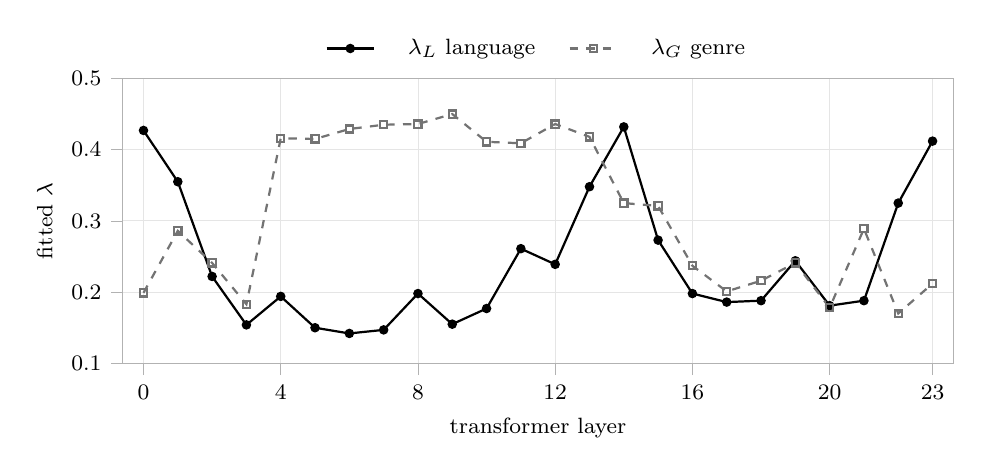
\begin{tikzpicture}
\begin{axis}[
  width=\columnwidth, height=5.2cm,
  font=\footnotesize,
  xlabel={transformer layer}, ylabel={fitted $\lambda$},
  xlabel near ticks, ylabel near ticks,
  xmin=-0.6, xmax=23.6, ymin=0.10, ymax=0.50,
  xtick={0,4,8,12,16,20,23}, ytick={0.1,0.2,0.3,0.4,0.5},
  tick align=outside, tick pos=left,
  axis line style={gray!60}, tick style={gray!60},
  grid=major, grid style={gray!20, line width=0.3pt},
  legend style={at={(0.5,1.03)}, anchor=south, legend columns=2,
                draw=none, fill=none, column sep=1em},
  legend cell align=left,
]
\addplot[black, thick, mark=*, mark size=1.3pt] coordinates {
 (0,0.427) (1,0.355) (2,0.222) (3,0.154) (4,0.194) (5,0.150)
 (6,0.142) (7,0.147) (8,0.198) (9,0.155) (10,0.177) (11,0.261)
 (12,0.239) (13,0.348) (14,0.432) (15,0.273) (16,0.198) (17,0.186)
 (18,0.188) (19,0.244) (20,0.181) (21,0.188) (22,0.325) (23,0.412)};
\addlegendentry{$\lambda_L$ language}
\addplot[black!55, thick, dashed, mark=square, mark size=1.3pt,
         mark options={solid}] coordinates {
 (0,0.199) (1,0.286) (2,0.241) (3,0.183) (4,0.416) (5,0.415)
 (6,0.429) (7,0.435) (8,0.436) (9,0.450) (10,0.411) (11,0.409)
 (12,0.436) (13,0.418) (14,0.325) (15,0.321) (16,0.237) (17,0.201)
 (18,0.216) (19,0.241) (20,0.178) (21,0.289) (22,0.170) (23,0.212)};
\addlegendentry{$\lambda_G$ genre}
\end{axis}
\end{tikzpicture}
\caption{The per-layer fit, initialised at the global optimum $(0.3,0.3)$. The
language module is wanted at the edges of the network and the genre module in
its middle; across depth the two profiles run opposite to each other, though
with 24 points the correlation ($r=-0.28$) does not by itself exclude zero.
Forty-eight free parameters on one seed: the shape is reported as exploratory.}
\label{fig:profundidad}
\end{figure}

\paragraph{The two modules separate by depth.} The per-layer fit improves test
by a further $-0.0019$, and the two profiles come out inverted
(Figure~\ref{fig:profundidad}): the language module is wanted at the two
terminal layers --- adjacent to the embedding matrix and the output vocabulary
--- and the genre module in the interior. The surface properties of a language
live next to the embeddings and the output vocabulary, and the interior is where
the more abstract, style-like structure lives. The window is not one we chose:
it falls out of a fit that was free to place $\lambda_L$ anywhere. We report the
profile as exploratory all the same, and the $-0.0019$ as a number we would not
defend alone.

\section{Analysis}

\subsection{Where the gains and losses come from}
\label{sec:perfil}

Per-token NLL for each system on the test split, decomposed by position, token
class, and corpus frequency --- the last exactly, since the training blocks are
still in memory and can be counted. Bytes are attributed token by token, which
recovers 84\% of the true count because decoding tokens in isolation loses
leading spaces; that loss falls almost entirely on word-initial tokens, so
comparisons across groups carry a bias we have not bounded.

\begin{figure}[t]\centering
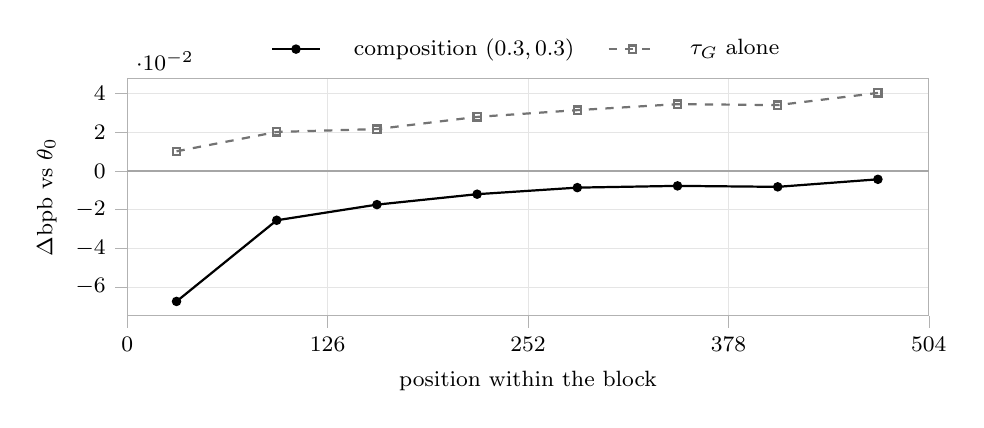
\begin{tikzpicture}
\begin{axis}[
  width=0.97\columnwidth, height=4.6cm,
  font=\footnotesize,
  xlabel={position within the block}, ylabel={$\Delta$bpb vs $\theta_0$},
  xlabel near ticks, ylabel near ticks,
  xmin=0, xmax=504, ymin=-0.075, ymax=0.048,
  xtick={0,126,252,378,504}, ytick={-0.06,-0.04,-0.02,0,0.02,0.04},
  yticklabel style={/pgf/number format/fixed,
                    /pgf/number format/precision=2},
  tick align=outside, tick pos=left,
  axis line style={gray!60}, tick style={gray!60},
  grid=major, grid style={gray!20, line width=0.3pt},
  legend style={at={(0.5,1.03)}, anchor=south, legend columns=2,
                draw=none, fill=none, column sep=1em},
  legend cell align=left,
]
\addplot[gray!70, line width=0.4pt, forget plot] coordinates {(0,0) (504,0)};
\addplot[black, thick, mark=*, mark size=1.3pt] coordinates {
 (31,-0.0675) (94,-0.0255) (157,-0.0174) (220,-0.0120)
 (283,-0.0086) (346,-0.0077) (409,-0.0082) (472,-0.0043)};
\addlegendentry{composition $(0.3,0.3)$}
\addplot[black!55, thick, dashed, mark=square, mark size=1.3pt,
         mark options={solid}] coordinates {
 (31,0.0102) (94,0.0202) (157,0.0217) (220,0.0280)
 (283,0.0315) (346,0.0346) (409,0.0341) (472,0.0404)};
\addlegendentry{$\tau_G$ alone}
\end{axis}
\end{tikzpicture}
\caption{Per-token $\Delta$bpb against the backbone, by position within the
512-token block, in eighths. The composition's gain is almost entirely spent in
the first eighth, while the genre module on its own grows steadily more damaging
as context accumulates. Negative is better than $\theta_0$.}
\label{fig:posicion}
\end{figure}

\paragraph{The gain lives at the cold start, and the damage where the corpus is
thin.} The composition's gain is concentrated in the opening of the block and
the genre module's damage in its close (Figure~\ref{fig:posicion}): with little
left context the model falls back on its priors, and that is what the modules
supply; once the evidence is in, an over-scaled prior only gets in the way. The
fall is a cliff rather than a slope --- 62\% of the gain is gone by the second
eighth --- so what the modules buy is a way to start, not a better model of the
text throughout. On the frequency
axis, $\tau_L$ costs $+0.005$ bpb on tokens its own corpus saw more than a
thousand times and between $+0.043$ and $+0.082$ on everything else --- up to
seventeen times more. The rate is not monotone in rarity and most of the damage
in absolute terms still sits in the mid-frequency bins, but the contrast between
the top bin and the rest is large and one-directional: the confound is not a
uniform fog.

\paragraph{The loss is register-specific, and there is no division of labour.}
The tokens $\tau_L$ damages most are the comma and the em dash, then \tec{vi}
(`we'), the full stop, the semicolon, then \tec{sade} (`said'), \tec{då},
\tec{han}, \tec{mig}. Administrative Swedish has no dialogue, no first person
and no verb of speech, and the module trained on it degrades the backbone on
precisely the tokens that mark narrative prose. What we do \emph{not} find is
the tidy story in which genre supplies lexis and language supplies morphology:
both modules damage word-initial tokens by almost exactly the same amount
($+0.025$ against $+0.024$ bpb, on 78\% of the bytes, that fraction taken from
exact character spans rather than from the token-by-token attribution). And one
caveat is large
enough to state as a result: the newline byte alone accounts for \textbf{27\% of
the composition's entire gain} in bits, eight times the next token. More than a
quarter of our headline number is line-break placement, which is a property of
how this corpus was segmented at least as much as it is genre. Setting it aside, what
remains is function words and typography.

\subsection{Three probes into where the modules act}
\label{sec:interp}

The three probes are: project one module's subspace out of the other in weight
space, which is the operator of Section~\ref{sec:comp}; measure the alignment of
the two modules' activation displacements; and remove from each module its
component along the other factor's axis, in state space. The middle one is a
measurement; the other two are interventions, and are reported by what they buy.

\paragraph{The modules are aligned in representation space, and the alignment
cannot explain the scale.} The null here is not the one of
Section~\ref{sec:comp}: principal-angle cosines are singular values with chance
at $\sqrt{r/d}$, whereas these carry a sign and average \emph{zero} for
independent pushes. Write $\delta_L$ for the displacement a module produces in
the hidden states --- $h(\tau_L)-h(\theta_0)$ at the same input --- and
$\delta_G$ for the other. Over 2{,}048 vectors per layer their mean cosine $c$
is $+0.132$, against a scale of $1/\sqrt{2048}=0.022$ for a single random cosine
in the width of the residual stream: six times larger, and far outside what
sampling noise could produce. So the two modules push the activations in substantially the same
direction while writing into near-orthogonal weight coordinates. That alignment
implies a scale. Taking the two displacements to have the same norm
$\lVert\delta\rVert$, the projection of $\lambda(\delta_L+\delta_G)$ onto
$\delta_L$ is $\lambda\lVert\delta\rVert(1+c)$, so the $\lambda$ that keeps the
shared part from being counted twice --- the one the double-counting account
calls for --- is $1/(1+c)$, here $0.88$. The fitted optimum is $(0.3,0.3)$: over $c\in[0,1]$ the
predicted scale never falls below one half, and reaching three tenths would need
$c=2.33$. Whatever forces $\lambda$ down is not the double-counting the
geometric account posits.

\paragraph{The confound is a measurable direction --- and it is the only thing
the axes see.} We build two axes from backbone centroids --- mean hidden states
over a set of text --- that differ in one factor at a time: genre as \emph{sv
literary} $-$ \emph{sv legal} (positive $=$ more literary), language as
\emph{non-sv literary} $-$ \emph{sv literary} (positive $=$ less Swedish).
Holding the other factor fixed is what makes each difference a direction for its
own. The two share the sv-literary centroid with opposite signs and are
therefore not orthogonal, so displacements are fitted onto the plane by least
squares rather than projected axis by axis. Decomposed that way,
$\tau_L$ has a clearly negative genre coefficient ($-0.084$) --- it drags the
target towards the \emph{legal} pole, its confound --- and $\tau_G$ a clearly
positive language coefficient ($+0.048$), dragging it towards
\emph{non-Swedish}, its confound. But each module's coefficient on its
\emph{own} factor's axis is small or wrong-signed: $\tau_G$ scores $+0.001$ on
the genre axis, $\tau_L$ scores $+0.030$ on the language axis. Within this
plane, each module moves the target along the axis of what contaminates it and
not along the axis it is named after. That is the claim of Section~1 in its
strongest form, measured rather than inferred.

\paragraph{The intervention that follows, and why it fails.} Removing that
component --- folded into the $B$ factor of \tec{o\_proj} and \tec{down\_proj},
the two matrices writing into the residual stream, so the result is still a LoRA
adapter --- moves the test score by $-0.0001$ bpb. The axes come from the
target's validation split, so this probe is not parameter-free and we compare it
against the fitted $\lambda$, not the plain sum; we also fixed the variant to
report in advance rather than choose among the four we ran, though choosing the
best on test would not change the figure. The reason it fails is in the same
decomposition: the plane accounts for 2.1\% of $\lVert\delta\rVert^2$ on average
and at most 7.4\%, so there is almost nothing to remove. For a directional
correction to pay here, a probe would have to reach far more of the displacement
than ours did; that is a statement about our axes, not about the geometry.

\section{Limitations}

\emph{Everything here is translated text}: DGT is a
translation memory and \tec{opus\_books} novels with their translations, so the
target and both modules are translations, and these two datasets cannot separate
Swedish literary text from translated Swedish. \emph{One work, three times}: the
findings speak about one novel, with the consequences for sample size and for
segmentation already given in Sections~\ref{sec:eval} and~\ref{sec:perfil}. \emph{The modules are not
compute-matched}: 48.6M words of genre against 11.1M of language, a factor of
$4.4$, so wherever the language module contributes little we cannot separate
``this factor carries less'' from ``this module saw less text''. \emph{No norm-matched control}: we claim total displacement governs the
composition but never measured it, in state space, for the scaled single-module
systems --- one forward pass. \emph{No
direct-adaptation reference}: Section~\ref{sec:sup} argues only that such a run
can obscure the effect, which is a reason not to substitute it for the
composition and not a reason to omit it; as a normaliser we would reject it
anyway, since 14.9M free parameters and an unconstrained recipe make that
denominator a knob. \emph{One seed}: the paired measurement is precise because systems see
identical text, but training variance is unbounded and is plausibly the larger
of the two uncertainties here --- the intervals we do report bound the smaller
one.

\section{Conclusion}

Two modules trained independently, neither ever shown the target cell and
neither of any use to it on its own, nevertheless model that cell better than
the backbone once they are combined at the right scale --- and they do it with
no target data at all.

What decides that composition is how much the two updates move the model and
not where they move it. We probed the direction three times, across two spaces,
and recovered essentially nothing, while a single scalar per module did the
work.

What the geometry does show, and show cleanly, is the confound the protocol
forces on us: each module displaces the target along the axis of the factor it
was contaminated with rather than its own. That is the finding we would carry to
the next cell, because it is a property of the design and not of this one.

\begin{thebibliography}{99}\footnotesize
\setlength{\itemsep}{1pt}
\bibitem{salamandra2025} A. Gonzalez-Agirre, M. P\`amies, J. Llop, et al. 2025.
Salamandra Technical Report. arXiv:2502.08489.
\bibitem{hu2022} E. J. Hu, Y. Shen, P. Wallis, et al. 2022. LoRA: Low-Rank
Adaptation of Large Language Models. \emph{ICLR}.
\bibitem{ilharco2023} G. Ilharco, M. T. Ribeiro, M. Wortsman, et al. 2023.
Editing models with task arithmetic. \emph{ICLR}.
\bibitem{koehn2004} P. Koehn. 2004. Statistical Significance Tests for Machine
Translation Evaluation. \emph{EMNLP}.
\bibitem{martins2024} P. H. Martins, P. Fernandes, J. Alves, et al. 2024.
EuroLLM: Multilingual Language Models for Europe. arXiv:2409.16235.
\bibitem{qwen3} Qwen Team. 2025. Qwen3 Technical Report. arXiv:2505.09388.
\bibitem{wortsman2022} M. Wortsman, G. Ilharco, S. Y. Gadre, et al. 2022. Model
soups: averaging weights of multiple fine-tuned models improves accuracy without
increasing inference time. \emph{ICML}.
\end{thebibliography}

\end{document}
